\chapter*{Résumé étendu}
\addcontentsline{toc}{chapter}{Résumé étendu}

\selectlanguage{french}

Le matériau central de cette thèse est le nitrure de bore hexagonal. Depuis sa première synthèse en 1842 par William H. Balmain, le nitrure de bore existe sous différentes formes, cristallines ou amorphes. Il est utilisé dans l'industrie comme lubrifiant, ou bien dans des composants soumis à de fortes températures, du fait de sa grande stabilité thermique et chimique.

Sa forme hexagonale (hBN) attire beaucoup l'attention des chercheurs en physique de la matière condensée depuis les vingt dernières années, depuis la synthèse de cristaux à haute pureté par Taniguchi et Watanabe en 2004. Cette forme a un réseau cristallin hexagonal, constitué de feuillets empilés les uns sur les autres, ou les atomes de bore et d'azote sont alternés aux sommets des hexagones et sont liés par des liaisons hybrides $sp^2$. Ce cristal est très similaire au graphite.
Le polytype le plus stable a un empilement dit AA', c'est-à-dire qu'un atome de bore est superposé à un atome d'azote du feuillet du dessous. C'est principalement ce polytype qui sera étudié dans cette thèse notamment dans le Chapitre 3. Il existe d'autres polytypes en fonction de l'empilement. Nous pouvons mentionner la forme dite Bernal (bBN) qui a un empilement AB, c'est-à-dire qu'un atome de bore est au-dessus du centre d'un hexagone du feuillet inférieur. Ce polytype sera étudié à la fin du Chapitre 4.
Les polytypes hBN et bBN sont des isolants avec des gaps d'énergie indirects autour de 6 eV. Cependant, la première caractérisation optique du hBN à haute pureté par Taniguchi et Watanabe a révélé que l'intensité de luminescence du hBN est bien plus haute que d'autres matériaux à gaps indirects comme le diamant, et comparable à celle de matériaux à gaps directs comme l'oxide de zinc. Ceci a conduit à un débat dans la communauté scientifique sur la nature directe ou indirecte du hBN massif. Aujourd'hui grâce à l'évolution technologique des appareils de mesure et grâce à des simulations \textit{ab initio}, il est acquis que ce matériau possède un gap indirect. Sa forte luminescence est due à un fort couplage entre les excitons et les vibrations du réseau cristallin, ce qui permet aux excitons noirs de se recombiner de façon radiative, en amplifiant l'intensité de luminescence. 

Tout comme le graphite, il est possible d'exfolier mécaniquement un ou plusieurs feuillets afin d'obtenir un crystal d'une épaisseur finie, allant jusqu'à une couche monoatomique. La monocouche de nitrure de bore hexagonal (mBN) a un paramètre de maille extrêmement proche de celui du graphène, qui fait l'objet d'énormément de recherches dues à ses propriétés remarquables. Il est ainsi un candidat de choix comme substrat ou matériau d'encapsulation sans contrainte pour le graphène, qui joue en plus le rôle de barrière de passivation. Il a été montré qu'il pouvait décupler la mobilité des électrons dans le graphène.
Du fait de son caractère isolant ainsi que sa transparence dans le domaine visible, le mBN peut également améliorer les propriétés optiques des dichalcogénures de métaux de transitions,
sans altérer leurs propriétés électroniques, ou bien agir comme isolant diélectriques entre deux matériaux pour contrôler leur couplage électrique.
En combinant différents matériaux en deux dimensions, avec ou sans contrainte, avec ou sans rotation entre les feuillets, les possibilités d'hétérostructures sont infinies et les propriétés optiques et électroniques peuvent être ajustées presque à volonté. Pour toutes ces raisons, le mBN est un matériau de choix dans l'élaboration de composants opto-électroniques. 

Pour mesurer les propriétés optiques d'un feuillet monoatomique, il faut descendre à température cryogénique et avoir des appareils avec des résolutions très fines. C'est pourquoi les mesures précises de luminescence de mBN sont apparues dans la littérature scientifique seulement récemment. De plus, ces mesures contiennent des structures différentes d'un spectre à l'autre et leurs interprétations ne sont pas unanimes. \\

%
%   Chap 2 : theory
%
Après cette introduction générale, le Chapitre 2 contient la présentation du socle théorique nécessaire à nos calculs, qui commence par l'explication du problème à N-corps, essentiel dans tous les domaines de la physique de la matière condensée. D'un point de vue théorique, l'Hamiltonien qui décrit le système d'électrons et d'ions qui constitue les solides ou les molécules peut s'écrire en une somme de six termes. Ce qui peut sembler assez simple est pourtant insolvable dès que le nombre d'électrons et d'ions considérés dépasse une dizaine. En effet, bien que certains termes ne posent pas de problème particulier à calculer comme les énergies cinétiques totales des électrons ou des ions, les autres termes peuvent être immensément plus compliqués, comme l'interaction électron-électron, qui est une interaction à deux corps. La complexité de ce terme fait que l'on doit recourir à des simplifications et des approximations pour réussir à calculer les propriétés des solides qui nous intéressent. Bien qu'il soit possible de recourir à des modèles et de décrire certaines propriétés par des paramètres, l'approche choisie dans cette thèse est dite \textit{ab initio}, c'est-à-dire que les seules données initiales sont les numéros atomiques des atomes composant le crystal ainsi que leurs positions. Dans cette approche, il faut s'assurer que les approximations faites ne soient pas trop restrictives et que toute la physique des phénomènes que nous tentons de reproduire soit incluse. Cela peut mener à une complexité à la fois dans la formulation théorique, mais aussi dans l'implémentation numérique dans les codes de simulation. En général, les temps de calculs \textit{ab initio} sont plus longs que ceux des modèles. Toutefois du point de vue de l'utilisateur des codes de simulation, la tâche est simplifiée car il suffit seulement de préciser en entrée le type de cristal à étudier et de lire les sorties produites par les codes. 

La première approximation est celle de Born-Oppenheimer, qui consiste à découpler le mouvement des ions et celui des électrons. On considère que les électrons sont toujours dans l'état fondamental lorsqu'on calcule le mouvement des ions, et les positions ioniques sont un paramètre dans l'Hamiltonien des électrons.

La première théorie décrite ici est celle de la fonctionnelle de la densité (DFT), élaborée dans les années 1960 par Hohenberg, Kohn et Sham. Celle ci a pour but de calculer la densité électronique dans l'état fondamental du système. On peut montrer que l'énergie totale du système dépend de la densité électronique. L'idée pour calculer la densité est de construire un système auxiliaire qui aurait la même densité dans l'état fondamental que le système réel qui nous intéresse, mais dont les électrons sont indépendants les uns des autres. Leur interaction est remplacée par un champ moyen qui contient les effets électrostatiques classiques ainsi que les effets quantiques d'échange et de corrélation. Ce champ moyen est le potentiel de Kohn-Sham. Il est présent dans une équation de Schrödinger, appelée l'équation de Kohn-Sham, pour chaque particule indépendante du système auxiliaire. Cependant l'expression analytique de ce potentiel dépend de la densité électronique, comme montré par Kohn et Sham. A son tour, la densité peut être calculée en sommant les modules carrés des fonctions d'ondes solutions des équations de Kohn-Sham. Nous voyons ici que pour obtenir la densité électronique, il faut résoudre les équations de Kohn-Sham de façon autocohérente, en partant d'une densité hypothétique et en convergeant à chaque itération vers la bonne densité. Une fois que la densité ne varie pas plus qu'un seuil arbitraire à chaque itération, le calcul s'arrête et nous pouvons obtenir l'énergie totale de l'état fondamental du système.

Cette théorie est en principe exacte, mais le potentiel d'échange-correlation n'a pas d'expression analytique et est impossible à calculer avec précision. Pour cette raison, il faut l'approximer afin de rendre sa dépendance en la densité calculable. Différentes approximations existent telles que l'approximation de la densité locale (LDA) ou l'approximation du gradient généralisé (GGA). Chaque approximation a ses avantages et ses inconvénients, et se rapprochent toutes plus ou moins du vrai potentiel d'échange-corrélation. De plus le potentiel ionique dans lequel évoluent les particules indépendantes, qui contient une divergence autour de la position des ions, est lui aussi approximé par des pseudopotentiels pour supprimer cette divergence et accélérer les calculs. Ces potentiels approximés sont appelés pseudopotentiels. 

Afin de pouvoir diagonaliser l'Hamiltonien et résoudre les équation de Kohn-Sham, il faut choisir une base dans laquelle exprimer les fonctions d'ondes. La base que nous utilisons dans cette thèse est la base des ondes planes. Celle-ci a la particularité de bien s'accorder avec le théorème de Bloch qui décrit les électrons dans des cristaux périodiques. Ici les électrons de Bloch sont décrits par une combinaison linéaire d'ondes planes, et possèdent donc un moment et un vecteur d'onde.

Il faut toutefois insister sur le fait que les valeurs propres des équations de Kohn-Sham ne sont pas les états d'énergie des vrais électrons du système. Ce sont les niveaux d'énergie du système auxiliaire, qui n'ont pas de réelle signification physique. Toutefois, si les approximations sont suffisamment précises et que le calcul de densité est suffisamment convergé, les valeurs propres de Kohn-Sham peuvent donner un bonne approximation des niveaux d'énergies du vrai système, mais seulement pour les plus hauts états de valence. Le gap des semi-conducteurs et des isolants n'est jamais précis en DFT et il faut recourir à des théories plus précises pour décrire le gap et les états d'énergies excités du système.

Ceci est réalisé grâce à la théorie des perturbations à N-corps (MBPT). Cette théorie est basée sur la fonction de Green du système à N électrons. Cet object mathématique a le sens physique du propagateur à N particules, c'est à dire la probabilité qu'un électron introduit à l'instant $t_1$, à la position $r_1$ et avec le spin $\sigma_1$ se propage jusqu'à la position $r_2$ et avec le spin $\sigma_2$ au temps $t_2$. Dans cette thèse, la dépendance en spin n'est pas considérée donc elle est toujours implicite. Mathématiquement, la fonction de Green est la solution d'une équation différentielle dont le terme de source est un delta de Dirac. Dans notre cas, c'est la solution de l'équation de Schrödinger contenant l'Hamiltonien électronique. La fonction de Green complète du système est une matrice multidimensionnelle, dont les deux premiers éléments de matrice sont la fonction de Green à une particule et la fonction de Green à deux particules. Beaucoup de quantités physiques intéressantes peuvent être extraites de ces fonctions, comme par exemple l'énergie totale du système d'électron corrélés. Plus intéressant dans notre cas, les pôles de la fonction de Green à une particule donnent les énergies d'excitation du système à N électron interagissant. On peut faire l'analogie entre les pôles de la fonction de Green à une particule et les spectres de photoémission ou de photoémission inversée. En effet, ces mesures consistent à mesurer l'énergie cinétique d'un électron arraché ou ajouté au système à N électrons, afin de déterminer les niveaux d'énergie existants. De façon équivalente, les pôles de la fonction de Green à N-1 électrons donnent les niveaux de valence du système, et ceux de la fonction de Green à N+1 électrons donnent les niveaux de conduction.

La fonction de Green à une ou deux particules est calculée en prenant en compte l'interaction avec tous les électrons. Les dérivations sont esquissées dans la partie 2.3 de la thèse. L'idée est d'ajouter une perturbation au système et de calculer les variations des différents potentiels grâce à la dérivée fonctionnelle par rapport à la perturbation. De cette façon et si l'on définit des nouvelles quantités physiques telles que la polarisabilité, la matrice diélectrique, la self-énergie ou encore l'interaction écrantée, on peut obtenir un système d'équations intégro-différentielles qui relient toutes ces quantités. Ce sont les équations d'Hedin, qui sont en principe exactes mais impossible à résoudre de façon analytique pour des systèmes réels. Pour simplifier la résolution, une des approximations les plus répandues consiste à négliger l'interaction électron-trou dans le vertex. De cette façon, la self-énergie se réduit au produit matriciel de la fonction de Green électronique $G$ et de l'interaction écrantée $W$, ce qui donne le nom d'approximation $GW$. Avec cette approximation, les équations d'Hedin peuvent être reformulées en terme de \textit{quasiparticules}, c'est-à-dire que les électrons ne sont plus considérés indépendants mais ``habillés'' par l'interaction avec les autres. Les énergies de ces quasiparticules sont données par les pôles de la fonction de Green électronique. Cela permet d'obtenir la structure de bandes électronique du système en meilleur accord avec l'expérience par rapport à la \acrshort{DFT}. Un lien peut également être établi entre les pôles de la fonction de Green et les énergies d'ionisation et l'affinité électronique du système. Ainsi on peut simuler les expériences consistant à ajouter ou à arracher un électron du système. Ces variations de charge sont appelées excitations neutres, qui sont ainsi bien décrites par l'approximation $GW$.

En revanche, les excitations neutres, c'est-à-dire qu'un électron du système est promu à une bande de conduction mais ne quitte pas le cristal, nécessitent de considérer l'interaction électron-trou, négligée plus haut. A cette fin, nous considérons une équation de Dyson pour la fonction de Green à deux particules. Elle est appelée l'équation de Bethe-Salpeter (BSE) et décrit la propagation de paires électron-trou liés par l'interaction de Coulomb. Une telle paire liée est un nouveau type de quasiparticule appelée \textit{exciton}. Moyennant quelques approximations décrites dans le Chapitre 2, la BSE peut être reformulée en un Hamiltonien à deux particules écrit dans la base des excitons. Ses valeurs propres sont les énergies des excitons et les coefficients du changement de base sont les vecteurs propres des excitons. 

La description des excitons est essentielle afin de reproduire correctement les spectres optiques obtenus expérimentalement. Il est possible d'écrire les fonctions de réponse du système dans la base des excitons, ainsi que la fonction diélectrique microscopique. Ensuite, on peut obtenir la partie imaginaire de la fonction diélectrique macroscopique, qui est directement proportionnelle à l'observable mesuré dans les mesures d'absorption optique. L'inclusion des effets excitoniques permet de simuler des spectres très ressemblants avec l'expérience.

Pour simuler des spectres de luminescence en revanche, une formulation \textit{ab initio} nécessiterait la description de phénomènes hors équilibre concernant l'interaction d'excitons, phonons et photons. Bien que certaines approchent aillent dans ce sens, cela est hors de la portée de cette thèse. En revanche, nous supposons que les systèmes que nous simulons sont dans une situation de quasi-équilibre, et que l'absorption et l'émission de lumière sont en équilibre dans un régime permanent. Cette approximation nous permet d'utiliser la relation de van Roosbroeck--Shockley qui permet de calculer le taux d'émission spontanée à partir du taux d'absorption. Le seul inconvénient est qu'il faut introduire un paramètre pour décrire le quasi-équilibre et le fait que les particules excitées ne sont pas décrite par la même température que le réseau. Dans cette thèse nous avons fait le choix de la fonction de Boltzmann qui donne de bons résultats pour une faible densité d'excitons. Il nous a donc fallu introduire une température excitonique que nous avons fitté sur des mesures expérimentales. C'est le seul paramètre parmi tous nos calculs \textit{ab initio}.

Nous présentons ensuite comment décrire les vibrations du réseau cristallin. Nous considérons que les atomes vibrent autour de leur position d'équilibre comme des oscillateurs harmoniques quantiques. Un quantum de vibration est appelé un \textit{phonon}, c'est une excitation collective avec une fréquence et un vecteur d'onde donnés. Nous présentons dans la section 2.5 une théorie basée sur un perturbation de la \acrshort{DFT}, appelée théorie de la perturbation de la fonctionnelle de la densité (DFPT). Elle permet de calculer les fréquences et vecteurs propres de phonons dans une cellule unité. Les fréquences dépendent des vecteurs d'onde ou de façon équivalente du moment, et on peut obtenir les courbes de dispersion de chaque mode de phonon. 

Ensuite, le problème des vibrations des atomes et le problème électronique sont regroupés de nouveau pour obtenir le couplage électron-phonon. Nous pouvons le formuler en seconde quantification. Ce sera un élément clé dans la construction du couplage exciton-phonon étudié dans cette thèse. 
\begin{figure}[H]
	\vspace{0.2cm}
	\setcapindent{2em}
	\centering
	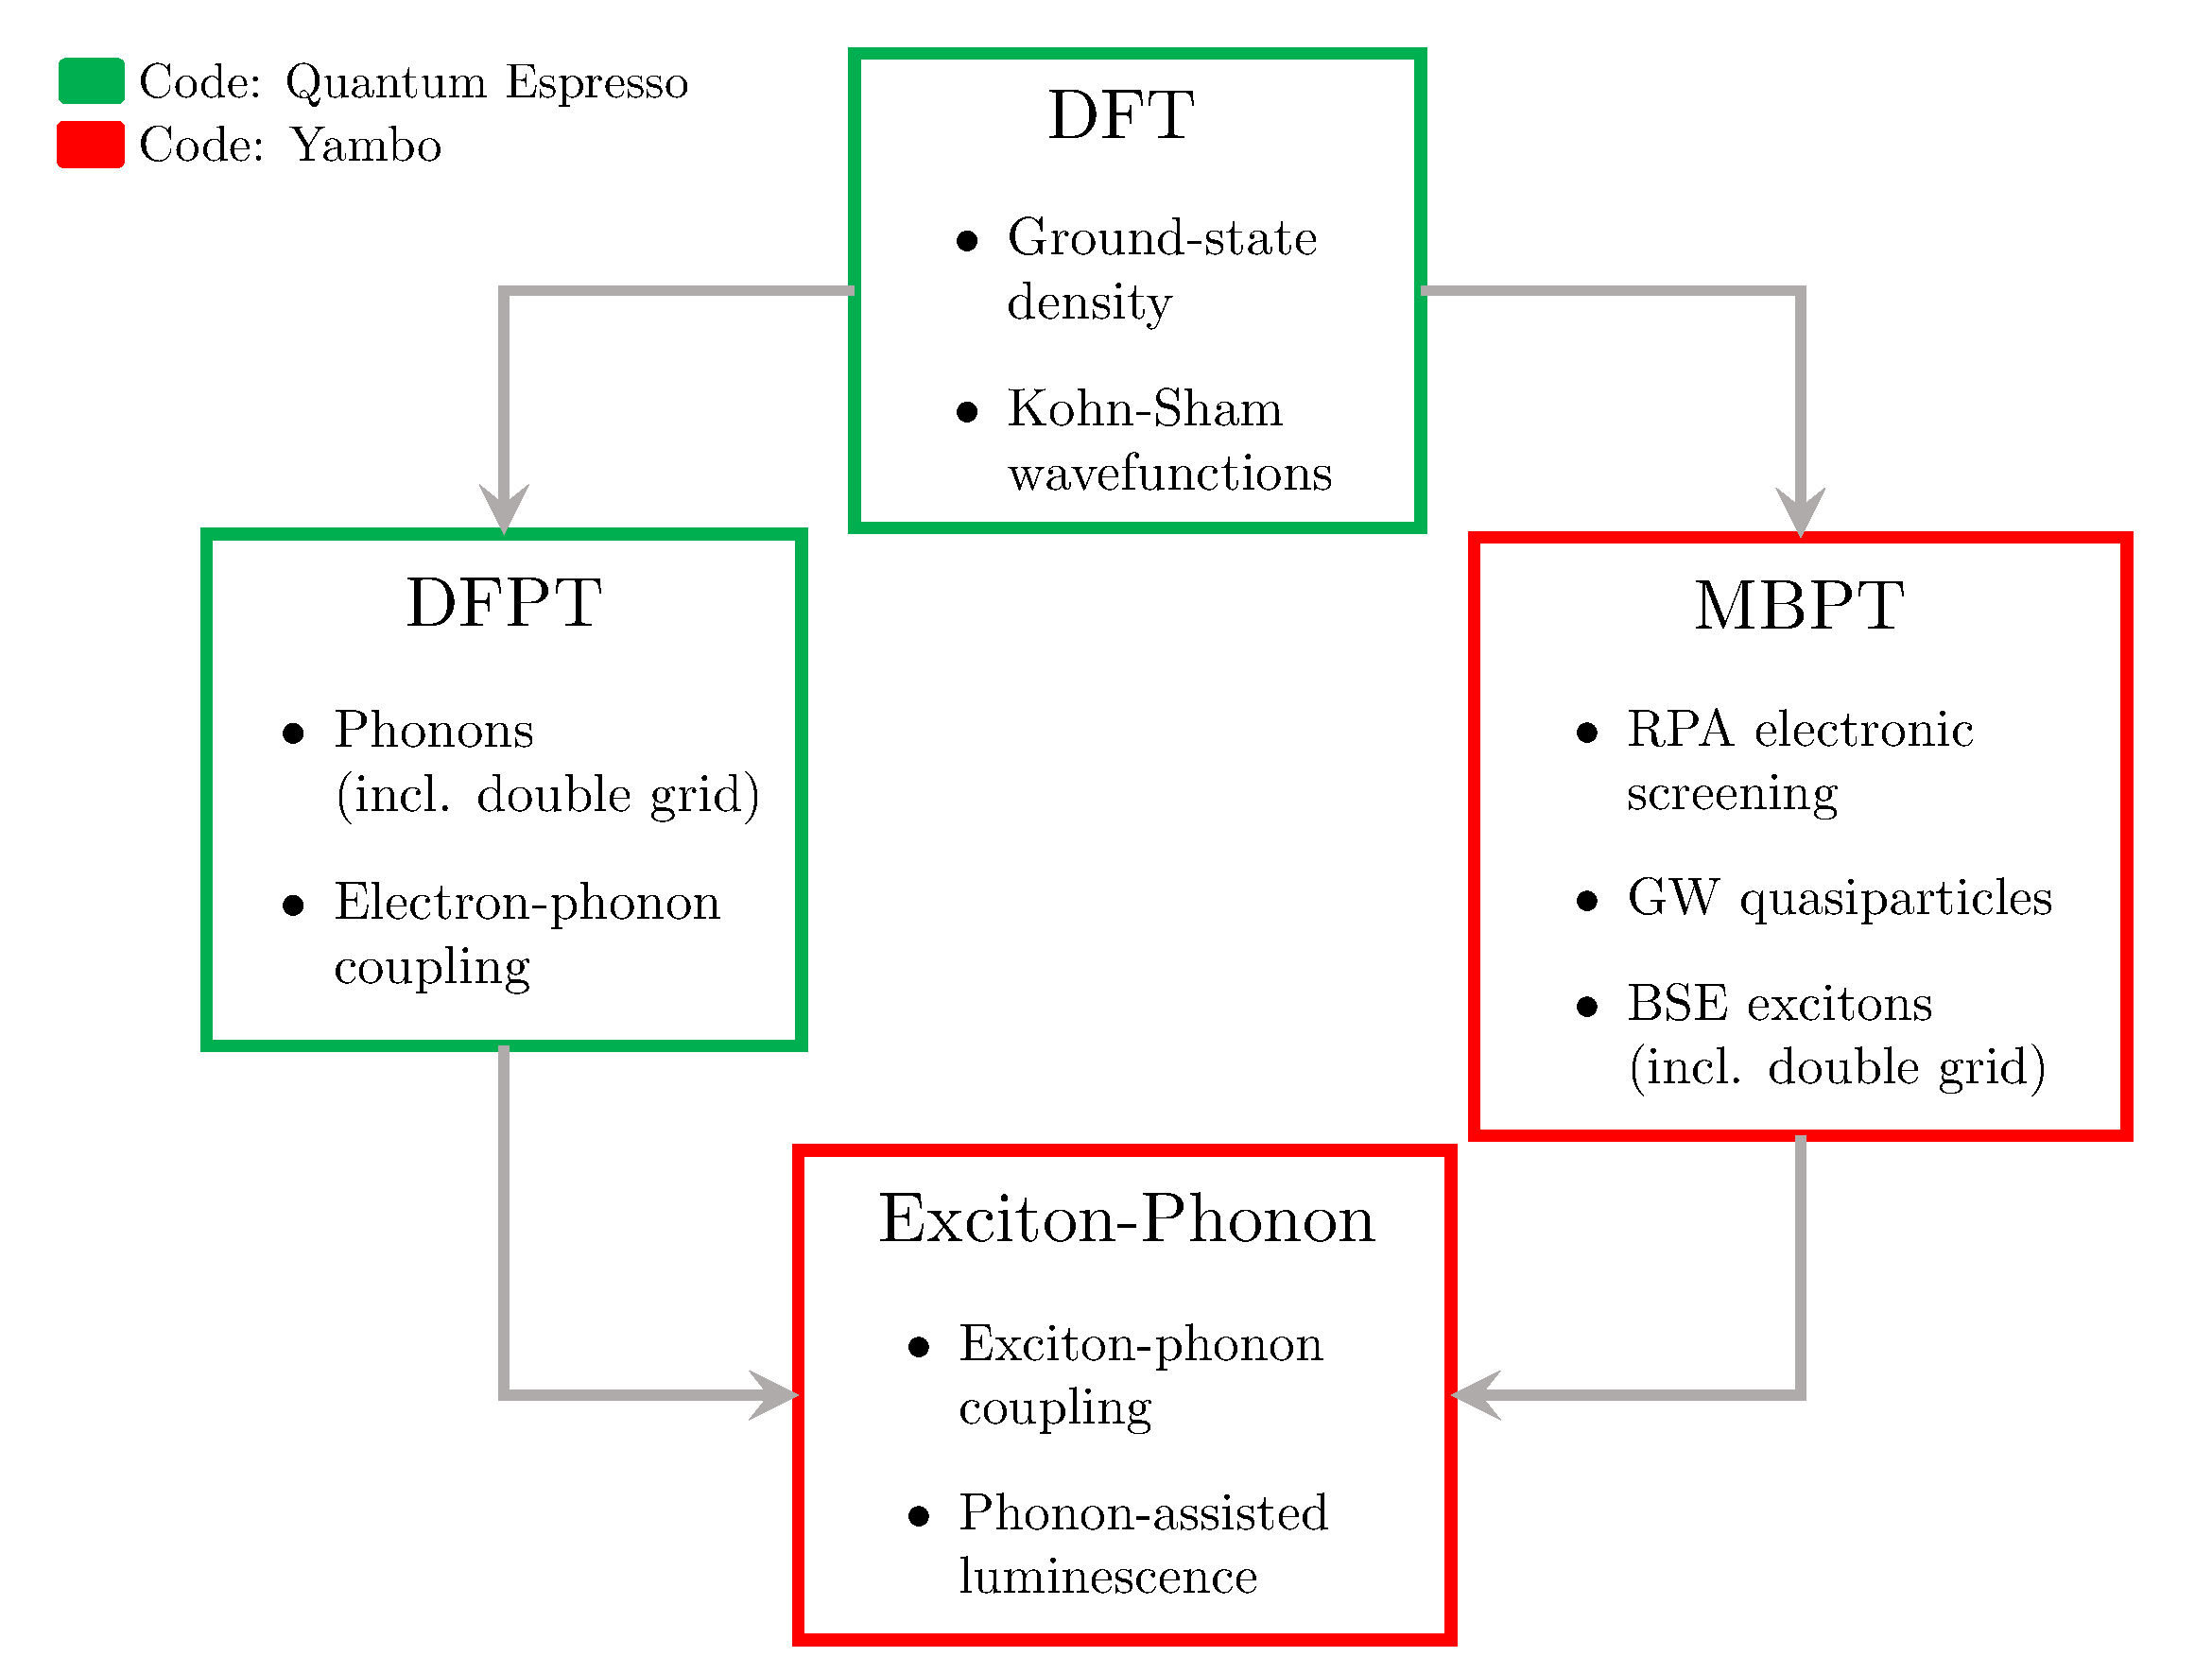
\includegraphics[width=0.8\textwidth]{intro/workflow_detailed.pdf}
	\caption{Schéma du processus de calcul du couplage exciton-phonon et de la luminescence assistée par les phonons. Les cadres verts et rouges indiquent l'utilisation de \textsc{Quantum ESPRESSO} et \yambo~comme codes de simulation, respectivement.}
	\label{fig:workflow_fr}
\end{figure}
Un schéma du processus de calcul est présenté dans la Fig. \ref{fig:workflow_fr}, qui contient également le nom des codes de simulation utilisés.\\


%
%   Chap 3 : strain
%
Après avoir présenté l'état de l'art théorique, nous passons aux résultats de cette thèse. Dans le Chapitre 3 nous reportons nos résultats obtenus sur le hBN massif soumis à une déformation uniaxiale. Nous commençons par présenter les motivations expérimentales. Nous avons tenté de reproduire la variation d'intensité relative des différents pics dans les spectres de cathodoluminescence d'un feuillet de hBN déposé sur un substrat nanostructuré qui induit une déformation de l'échantillon. A différents endroits du cristal, les pics correspondants à des transitions assistées par des phonons acoustiques voient leur intensité augmenter par rapport aux pics des phonons optiques, en corrélation avec la déformation de l'échantillon. Pour simuler ces conditions, nous appliquons une déformation uniaxiale à un cristal de hBN massif. Nous avons étudié l'effet sur les propriétés électroniques, phononiques et excitoniques pour des valeurs allant d'une compression de 2.5\% à un étirement de 2.5\% de la longueur à l'équilibre.
Nous observons que la déformation induit une brisure de symétrie et que la zone de Brillouin n'est plus un hexagone parfait. Les fréquences de phonons sont augmentées ou diminuées, suivant les modes considérés et la valeur de déformation appliquée. Il en va de même pour les bandes électroniques. Nous proposons une interprétation en terme d'interaction inter-feuillets, qui dépend fortement de la distance entre les feuillets superposés et qui et modifiée avec la déformation. Nous constatons que la brisure de symétrie lève la dégénérescence dans les orbitales à extrémités des bandes de valence et conduction. Ceci les points de haute symétrie dans l'espace réciproque $K$ et $M$ non-équivalents aux points $K'$ et $M'$. Il y a donc quatre transitions non-équivalentes extrêmement proches en énergie. 

La levée de dégénérescence a également un effet sur les énergies des excitons. Nous observons que les deux excitons directs avec les plus basses énergies, qui sont doublement dégénérés à l'équilibre, se séparent et donnent quatre niveaux distincts. L'énergie des excitons directs décroissent pour des étirements et croissent pour des compressions. Pour les excitons indirects, qui ne sont pas dégénérés, la tendance n'est pas la même et leur énergie décroît pour toutes les valeurs de déformation. L'effet de la séparation des niveaux d'énergie est clairement visible sur le spectre d'absorption où l'on voit apparaître un deuxième pic, provenant de la séparation de l'exciton blanc en deux états. L'effet est également visible sur la fonction d'onde de ces deux nouveaux états : en effet les deux ne sont pas orientés suivant la même direction cristallographique.

Dans la section 3.5, nous présentons l'approche utilisée pour calculer l'effet des phonons sur les excitons. Le couplage est obtenu par une dérivée aux différences finies de la fonction de réponse ou des dipoles excitoniques, de façon équivalente. Cette dérivée permet de calculer le couplage des excitons à moments finis avec les modes de phonons ayant les mêmes moments. Il est donc nécessaire de construire des supercellules pour pouvoir capturer la périodicité des modes de phonons aux moments choisis. Dans notre cas et comme évoqué plus haut, il nous faut considérer toutes les transitions non-équivalentes donnant des excitons indirects à très proche énergie. Tout ceci nous conduit à présenter les spectres de luminescence à différente valeur de déformation dans la Fig. \ref{fig:Lum_vs_strain_fr}.
\begin{figure}[h!t]
	\vspace{0.2cm}
	\setcapindent{2em}
	\centering
	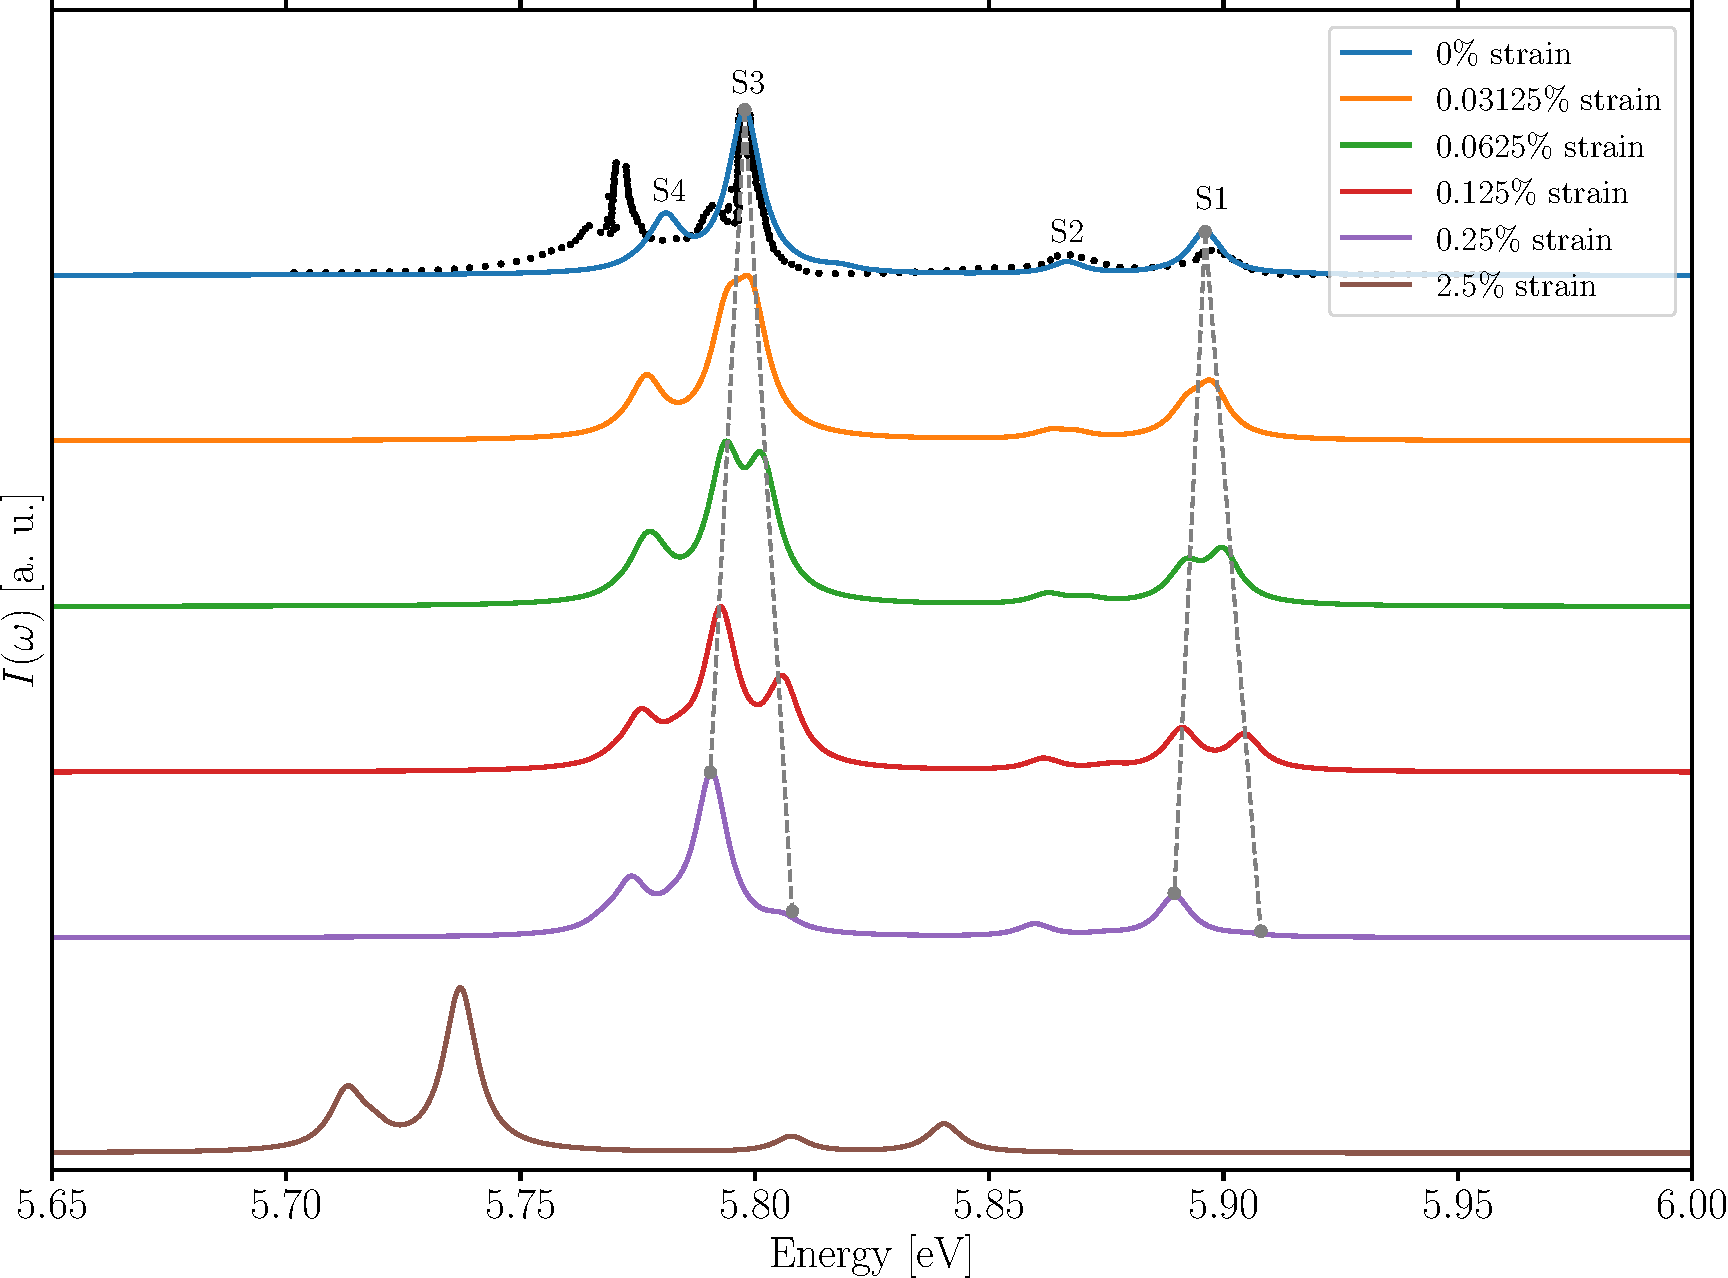
\includegraphics[width=0.8\textwidth]{Lum_vs_strain.pdf}
	\caption{Spectres de luminescence en fonction de la déformation, pour des valeurs choisies de compression. Les courbes sont déplacées verticalement par souci de clarté. Les données expérimentales sont reportés par les points noirs de la courbe du haut. Les spectres sont décalés en énergie pour correspondre à l'expérience. Les lignes pointillées sont un guide visuel.}
	\label{fig:Lum_vs_strain_fr}
\end{figure}

Ces résultats montrent un élargissement des répliques de phonon à faible valeur de déformation, ainsi qu'une faible augmentation de l'intensité des pics à haute énergie. Ceci est causé par l'inclusion des quatre transitions non-équivalentes proches en énergie. Nous voyons que ces pics se séparent de plus en plus avec l'augmentation de la compression, jusqu'à ce qu'un seul pic subsiste à -2.5\%, une compression relativement importante. Ces résultats vont dans le sens des mesures expérimentales mais l'accord n'est pas total. L'utilisation d'un nombre restreint de moments de phonons et d'excitons est une limitation. Il se peut aussi que des facteurs expérimentaux aient été négligés par notre méthode, comme le fait que la déformation ne soit pas nécessairement uniaxiale.\\


%
%   Chap 4 : mBN
%
Dans le Chapitre 4, nous présentons un approche pour calculer le couplage exciton-phonon qui permet de surpasser la méthode par différences finies. Nous utilisons la théorie des perturbations pour inclure de façon dynamique l'interaction électron-phonon à l'intérieur d'un Hamiltonien. Celui-ci contient les éléments de couplage exciton-phonon, qui sont construits à partir de quantités calculées \textit{ab initio} d'une part avec la BSE et en DFPT d'autre part. Ensuite, nous reformulons le problème pour obtenir une self-énergie décrivant l'interaction exciton-exciton médiée par des phonons. De cette façon nous pouvons écrire une fonction de réponse du système contenant une correction dynamique due à l'interaction avec les phonons. Cette correction dynamique est une avancée du point de vue théorique car elle permet d'obtenir les satellites de phonons dans les spectres optiques et surtout la renormalisation qu'ils causent à l'intensité des pics directs. De cette façon nous pouvons comparons l'intensité relative des processus directs et des transitions indirectes assistées par les phonons. Ceci s'accompagne d'une avancée sur le plan numérique étant donné que notre formulation comprend le couplage de tous les excitons avec tous les modes de phonons, sur toute l'étendue de la zone de Brillouin. 

Nous avons implémenté cette approche dans le code \yambo, et nous l'avons testée sur le hBN massif pour lequel nous pouvons nous comparer à une littérature expérimentale et théorique abondante. Notre spectre obtenu est en plutôt bon accord avec l'expérience pour la position des pics et l'intensité du doublet LA/TA. En revanche, l'intensité du doublet LO/TO est inversée par rapport à l'expérience. De plus nous constatons l'apparition d'un satellite causé par les phonons ZA/ZO, qui ne devrait pas être visible car interdit par symétrie. Nous attribuons ces problèmes à la façon dont nous construisons les éléments de matrice de couplage exciton-phonon. En effet, ceux-ci sont obtenus par le produit d'une quantité phononique et un quantité excitonique qui ne sont pas calculées avec la même phase de Kohn-Sham de départ. Ce problème peut être réglé en désactivant l'utilisation des symétries de la zone de Brillouin et en écrivant une interface avec un troisième code de simulation, comme l'a été montré après la publication de nos résultats par un collaborateur. Cependant, appliquer cette solution augmente considérablement le temps de calcul et surtout l'espace disque nécessaire pour obtenir le couplage exciton-phonon sans le problème des phases. Etant donné que les ordres de grandeur des intensités sont corrects, nous avons décidé de continuer et d'appliquer cette méthode au feuillet monoatomique de hBN (mBN).

Nous avons étudié les propriétés excitoniques du mBN en détail. La dispersion d'excitons contient un minimum global au point $K$, donnant un caractère indirect à ce matériau, en contradiction avec les mesures expérimentales. Cet exciton provient des transitions électroniques entre la bande de valence et les états quasi-libres à $Gamma$ dans l'approximation $GW$. Cette vallée excitonique pourrait être la plus peuplée et causer l'extinction du signal de luminescence. Après une étude de la fonction d'onde et du couplage exciton-phonon de cet état, nous avons décidé de ne pas utiliser l'approximation $GW$ et de rester au niveau DFT+BSE, où ce problème est non-existant. L'étude des éléments de couplage exciton-phonon résolue en moment nous montre que le couplage est maximal dans une petite région autour de $\Gamma$ et quasiment nulle aux bords de la zone de Brillouin.

Nous avons finalement calculé le spectre de luminescence du mBN libre. Nous l'avons comparé à trois spectres expérimentaux publiés récemment. Les structures apparaissant dans les trois spectres ne sont pas les mêmes et les interprétations sur leur origine diffèrent. Nous reportons nos résultats et leur comparaison aux spectres expérimentaux dans la Fig. \ref{fig:mBN_PL_fr}
\begin{figure}[H]
	\vspace{0.2cm}
	\setcapindent{2em}
	\centering
	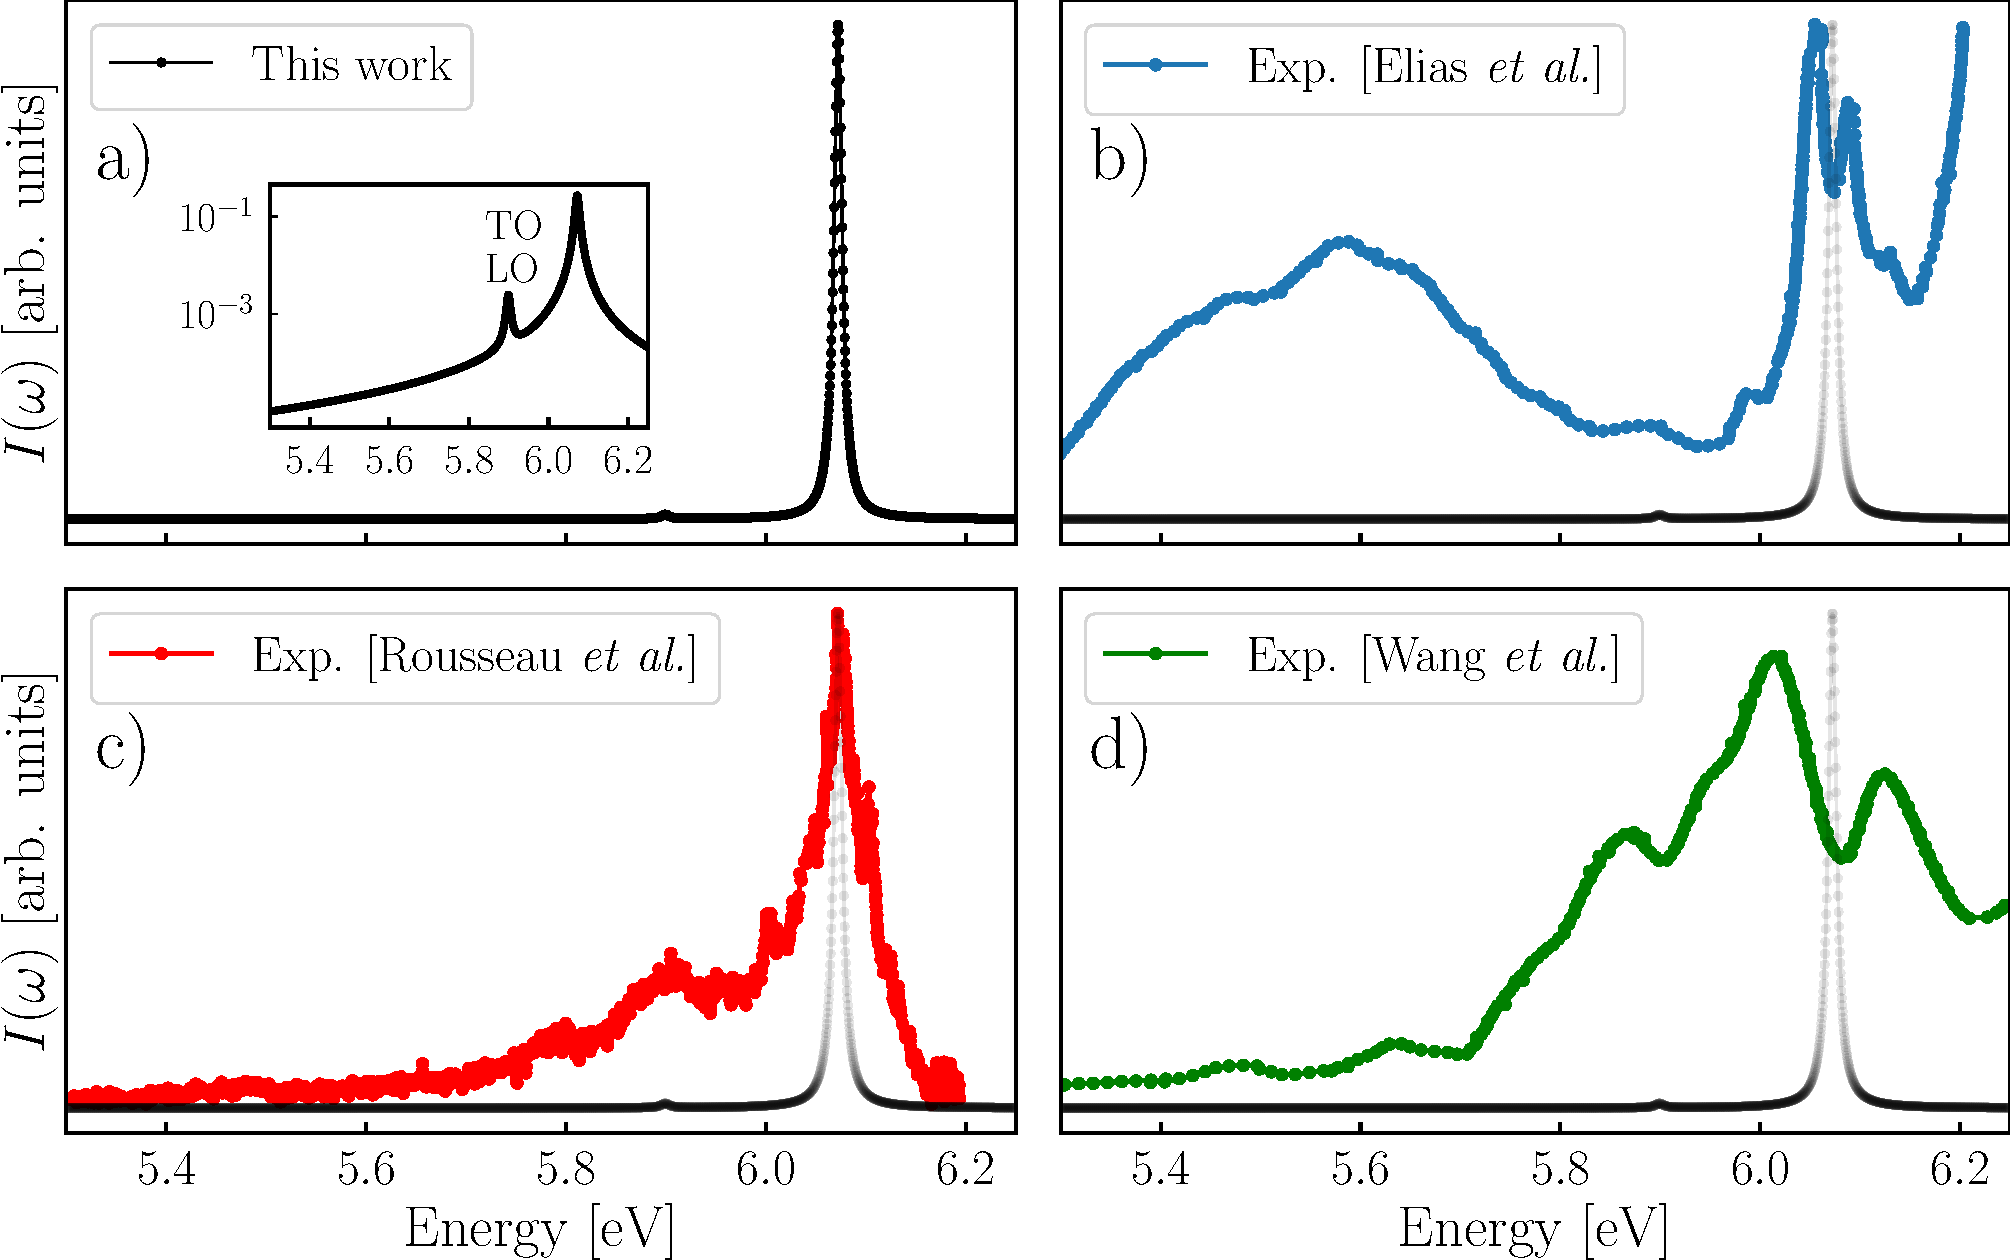
\includegraphics[width=0.8\textwidth]{hBN_monolayer_lum2.pdf}
	\caption{Spectre de luminescence calculé pour la monocouche de hBN (a) comparé aux résultats expérimentaux dans les Ref. \cite{elias2019direct}(b), Ref. \cite{rousseau2021monolayer}(c) et Ref. \cite{wang2022scalable}(d). Les spectres calculés ont été décalés en énergie pour s'accorder avec le pic principal du panel (c). Par souci de clarté, nous avons tracé le spectre calculé sur chaque panel. Dans l'encadré du panel (a) nous montrons la même courbe en échelle semi-logarithmique, qui révèle le satellite à moindre intensité.}
	\label{fig:mBN_PL_fr} 
\end{figure}

Grâce à notre méthode, nous pouvons comparer l'intensité relative du pic direct et des satellites de phonons, interprétés comme visibles dans certains des spectres. Nos résultats montrent un pic direct très intense. Nous voyons également un satellite issu du couplage entre l'exciton direct et des phonons optiques, mais dont l'intensité est inférieure à celle du pic direct de deux ordres de grandeur. Concernant des satellites issus du couplage de phonons avec un exciton indirect, nous n'en voyons pas apparaître. Nous pouvons donc éliminer l'hypothèse selon laquelle les structures expérimentales seraient des satellites de phonons. 

Nous avons étudié l'influence du substrat graphitique présent dans deux des trois expériences. Premièrement, l'influence du substrat augmente l'énergie de l'exciton problématique à $K$, ce qui valide notre choix de ne pas le considérer. Ensuite, nous avons modélisé l'effet de l'écrantage du substrat sur le spectre de luminescence avec un modèle. Nous en avons conclu que l'influence du substrat n'est probablement pas assez forte pour révéler les satellites de phonon. Cependant la complexité de nos calculs ne nous permet pas d'utiliser un modèle élaboré voire un calcul direct d'une épaisseur finie de substrat en plus du mBN. 

Enfin nous présentons dans la section 4.7 nos résultats préliminaires sur une autre phase de hBN, la phase Bernal qui correspond à un empilement AB des feuillets. Ce matériau a des gaps directs et indirects proches en énergie, ce qui pourrait révéler les signatures des excitons directs et des satellites de phonons de le même spectre de luminescence, à des intensités comparables. Nos premiers résultats tendent vers une luminescence directe, mais ceci fera l'objet d'une étude numérique plus poussée.\\


En conclusion cette thèse présente des spectres de luminescence calculés à partir de premiers principes. Deux méthodes différentes de calcul du couplage exciton-phonon ont été présentées et permettent d'obtenir une compréhension des processus donnant naissance aux structures dans les spectres.
Les résultats présentés ouvrent des perspectives d'amélioration à la fois théoriques et numériques dont certaines sont activement explorées.
Finalement, nous espérons que ces travaux peuvent avoir un impact et contribuer à l'élaboration de composants opto-électroniques ou photovoltaïques. 